\subsection{Repeater radio infrastructure}
The main task of the repeater is to receive weak signals and to re-transmit them with increased transmission power. Its radio infrastructure is supplied by electrical energy from the self-sufficient energy distribution system, for which the schematic structure is shown in the figure \ref{fig:tikz_rep_energy}. As it can be seen, an AE Solar AE195SMM6-36 PV generator with pre-mounted cables \circled{\footnotesize{A}}, a Victron BlueSolar MPPT 75/10 SCC and an Offgridtec Smart-Pro $12,8\mathrm{V}$ $50\mathrm{Ah}$ $\mathrm{LiFePO}_4$ battery are used. In addition, the cables \circled{\footnotesize{B}} and \circled{\footnotesize{C}}, which are designed for harsh environments, are used to connect these devices.
\begin{figure}[h!]
	\centering
	

\tikzset{every picture/.style={line width=0.75pt}} %set default line width to 0.75pt        

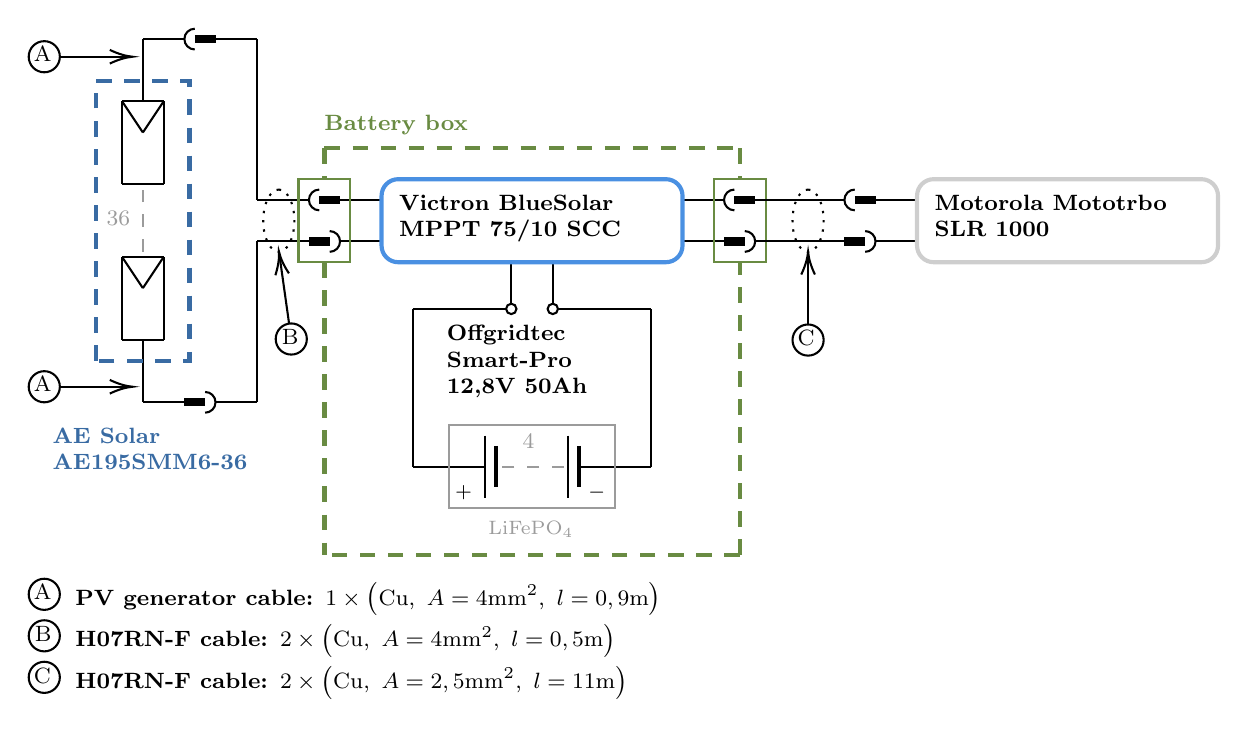
\begin{tikzpicture}[x=0.75pt,y=0.75pt,yscale=-1,xscale=1]
%uncomment if require: \path (0,440); %set diagram left start at 0, and has height of 440

%Straight Lines [id:da11510906097283446] 
\draw    (137,125) -- (162,125) ;
%Straight Lines [id:da5492120144829185] 
\draw    (137,145) -- (162,145) ;
%Straight Lines [id:da5723707691800957] 
\draw    (362,145) -- (342,145) ;
%Straight Lines [id:da24173928983034854] 
\draw    (362,125) -- (342,125) ;
%Straight Lines [id:da7288463432166432] 
\draw [line width=3]    (367,125) -- (377,125) ;
%Shape: Arc [id:dp807105785534799] 
\draw  [draw opacity=0] (367,120) .. controls (367,120) and (367,120) .. (367,120) .. controls (364.24,120) and (362,122.24) .. (362,125) .. controls (362,127.76) and (364.24,130) .. (367,130) -- (367,125) -- cycle ; \draw   (367,120) .. controls (367,120) and (367,120) .. (367,120) .. controls (364.24,120) and (362,122.24) .. (362,125) .. controls (362,127.76) and (364.24,130) .. (367,130) ;

%Straight Lines [id:da8769078095389509] 
\draw [line width=3]    (372,145) -- (362,145) ;
%Shape: Arc [id:dp8109222486657941] 
\draw  [draw opacity=0] (372,150) .. controls (372,150) and (372,150) .. (372,150) .. controls (374.76,150) and (377,147.76) .. (377,145) .. controls (377,142.24) and (374.76,140) .. (372,140) -- (372,145) -- cycle ; \draw   (372,150) .. controls (372,150) and (372,150) .. (372,150) .. controls (374.76,150) and (377,147.76) .. (377,145) .. controls (377,142.24) and (374.76,140) .. (372,140) ;

%Shape: Rectangle [id:dp029955475590352387] 
\draw  [color={rgb, 255:red, 105; green, 139; blue, 66 }  ,draw opacity=1 ][line width=0.75]  (382,115) -- (357,115) -- (357,155) -- (382,155) -- cycle ;
%Straight Lines [id:da46419191509797386] 
\draw    (177,145) -- (197,145) ;
%Straight Lines [id:da4717139050997601] 
\draw    (177,125) -- (197,125) ;
%Straight Lines [id:da7089947560118592] 
\draw [line width=3]    (167,125) -- (177,125) ;
%Shape: Arc [id:dp9143448676132002] 
\draw  [draw opacity=0] (167,130) .. controls (167,130) and (167,130) .. (167,130) .. controls (167,130) and (167,130) .. (167,130) .. controls (164.24,130) and (162,127.76) .. (162,125) .. controls (162,122.24) and (164.24,120) .. (167,120) -- (167,125) -- cycle ; \draw   (167,130) .. controls (167,130) and (167,130) .. (167,130) .. controls (167,130) and (167,130) .. (167,130) .. controls (164.24,130) and (162,127.76) .. (162,125) .. controls (162,122.24) and (164.24,120) .. (167,120) ;

%Straight Lines [id:da5416408978372171] 
\draw [line width=3]    (172,145) -- (162,145) ;
%Shape: Arc [id:dp8264873399510959] 
\draw  [draw opacity=0] (172,140) .. controls (172,140) and (172,140) .. (172,140) .. controls (172,140) and (172,140) .. (172,140) .. controls (174.76,140) and (177,142.24) .. (177,145) .. controls (177,147.76) and (174.76,150) .. (172,150) -- (172,145) -- cycle ; \draw   (172,140) .. controls (172,140) and (172,140) .. (172,140) .. controls (172,140) and (172,140) .. (172,140) .. controls (174.76,140) and (177,142.24) .. (177,145) .. controls (177,147.76) and (174.76,150) .. (172,150) ;

%Shape: Rectangle [id:dp42596657595685783] 
\draw  [color={rgb, 255:red, 105; green, 139; blue, 66 }  ,draw opacity=1 ][line width=0.75]  (157,115) -- (182,115) -- (182,155) -- (157,155) -- cycle ;
%Straight Lines [id:da8221096590097585] 
\draw    (212,177.5) -- (212,253.5) ;
%Straight Lines [id:da6364290852010983] 
\draw    (279.5,155) -- (279.5,175) ;
%Straight Lines [id:da7045932733322111] 
\draw    (259.5,155) -- (259.5,175) ;
%Shape: Circle [id:dp8158544821027223] 
\draw   (277,177.5) .. controls (277,176.12) and (278.12,175) .. (279.5,175) .. controls (280.88,175) and (282,176.12) .. (282,177.5) .. controls (282,178.88) and (280.88,180) .. (279.5,180) .. controls (278.12,180) and (277,178.88) .. (277,177.5) -- cycle ;
%Shape: Circle [id:dp11072945461222039] 
\draw   (257,177.5) .. controls (257,176.12) and (258.12,175) .. (259.5,175) .. controls (260.88,175) and (262,176.12) .. (262,177.5) .. controls (262,178.88) and (260.88,180) .. (259.5,180) .. controls (258.12,180) and (257,178.88) .. (257,177.5) -- cycle ;
%Straight Lines [id:da6164786002245375] 
\draw    (232,253.5) -- (212,253.5) ;
%Straight Lines [id:da9249854596615803] 
\draw [line width=0.75]    (247,238.5) -- (247,268.5) ;
%Straight Lines [id:da06155461019148012] 
\draw [color={rgb, 255:red, 155; green, 155; blue, 155 }  ,draw opacity=1 ] [dash pattern={on 4.5pt off 4.5pt}]  (285,253.5) -- (250,253.5) ;
%Straight Lines [id:da21626255863037636] 
\draw [line width=1.5]    (252,243.5) -- (252,263.5) ;
%Straight Lines [id:da8872957060723552] 
\draw [line width=0.75]    (287,238.5) -- (287,268.5) ;
%Straight Lines [id:da006768922210125705] 
\draw [line width=1.5]    (292,243.5) -- (292,263.5) ;
%Straight Lines [id:da03285061333508921] 
\draw    (247,253.5) -- (232,253.5) ;
%Straight Lines [id:da2369922648522118] 
\draw    (307,253.5) -- (292,253.5) ;
%Straight Lines [id:da7159577028550701] 
\draw    (327,253.5) -- (307,253.5) ;
%Shape: Rectangle [id:dp9889303998939478] 
\draw  [color={rgb, 255:red, 155; green, 155; blue, 155 }  ,draw opacity=1 ] (309.5,233.5) -- (309.5,273.5) -- (229.5,273.5) -- (229.5,233.5) -- cycle ;
%Straight Lines [id:da3151315575520983] 
\draw    (282,177.5) -- (327,177.5) ;
%Straight Lines [id:da3823389766737191] 
\draw    (212,177.5) -- (257,177.5) ;
%Straight Lines [id:da0570301114732914] 
\draw    (327,177.5) -- (327,253.5) ;
%Rounded Rect [id:dp777876749075382] 
\draw  [color={rgb, 255:red, 74; green, 144; blue, 226 }  ,draw opacity=1 ][line width=1.5]  (197,123) .. controls (197,118.58) and (200.58,115) .. (205,115) -- (334,115) .. controls (338.42,115) and (342,118.58) .. (342,123) -- (342,147) .. controls (342,151.42) and (338.42,155) .. (334,155) -- (205,155) .. controls (200.58,155) and (197,151.42) .. (197,147) -- cycle ;

%Straight Lines [id:da367136719676906] 
\draw [color={rgb, 255:red, 105; green, 139; blue, 66 }  ,draw opacity=1 ][line width=1.5]  [dash pattern={on 5.63pt off 4.5pt}]  (369.5,100) -- (369.5,115) ;
%Straight Lines [id:da16267897243027396] 
\draw [color={rgb, 255:red, 105; green, 139; blue, 66 }  ,draw opacity=1 ][line width=1.5]  [dash pattern={on 5.63pt off 4.5pt}]  (169.5,100) -- (369.5,100) ;
%Straight Lines [id:da8616987060550743] 
\draw [color={rgb, 255:red, 105; green, 139; blue, 66 }  ,draw opacity=1 ][line width=1.5]  [dash pattern={on 5.63pt off 4.5pt}]  (369.5,296) -- (169.5,296) ;
%Straight Lines [id:da36222203519709884] 
\draw [color={rgb, 255:red, 105; green, 139; blue, 66 }  ,draw opacity=1 ][line width=1.5]  [dash pattern={on 5.63pt off 4.5pt}]  (369.5,296) -- (369.5,155) ;
%Straight Lines [id:da6365045471237227] 
\draw [color={rgb, 255:red, 105; green, 139; blue, 66 }  ,draw opacity=1 ][line width=1.5]  [dash pattern={on 5.63pt off 4.5pt}]  (169.5,100) -- (169.5,115) ;
%Straight Lines [id:da6903074155504818] 
\draw [color={rgb, 255:red, 105; green, 139; blue, 66 }  ,draw opacity=1 ][line width=1.5]  [dash pattern={on 5.63pt off 4.5pt}]  (169.5,155) -- (169.5,296) ;
%Straight Lines [id:da4240086792410498] 
\draw    (435,125) -- (455,125) ;
%Straight Lines [id:da5129811579067403] 
\draw [line width=3]    (425,125) -- (435,125) ;
%Shape: Arc [id:dp06802688638649235] 
\draw  [draw opacity=0] (425,130) .. controls (425,130) and (425,130) .. (425,130) .. controls (422.24,130) and (420,127.76) .. (420,125) .. controls (420,122.24) and (422.24,120) .. (425,120) -- (425,125) -- cycle ; \draw   (425,130) .. controls (425,130) and (425,130) .. (425,130) .. controls (422.24,130) and (420,127.76) .. (420,125) .. controls (420,122.24) and (422.24,120) .. (425,120) ;

%Straight Lines [id:da13943249363545007] 
\draw    (376,125) -- (420,125) ;
%Straight Lines [id:da7940671666746317] 
\draw    (377,145) -- (420,145) ;
%Straight Lines [id:da47438289382255494] 
\draw [line width=3]    (430,145) -- (420,145) ;
%Shape: Arc [id:dp5577371328307759] 
\draw  [draw opacity=0] (430,140) .. controls (430,140) and (430,140) .. (430,140) .. controls (432.76,140) and (435,142.24) .. (435,145) .. controls (435,147.76) and (432.76,150) .. (430,150) -- (430,145) -- cycle ; \draw   (430,140) .. controls (430,140) and (430,140) .. (430,140) .. controls (432.76,140) and (435,142.24) .. (435,145) .. controls (435,147.76) and (432.76,150) .. (430,150) ;

%Straight Lines [id:da9662946735319131] 
\draw    (435,145) -- (455,145) ;
%Rounded Rect [id:dp6020333899040144] 
\draw  [color={rgb, 255:red, 206; green, 206; blue, 206 }  ,draw opacity=1 ][line width=1.5]  (455,123) .. controls (455,118.58) and (458.58,115) .. (463,115) -- (592,115) .. controls (596.42,115) and (600,118.58) .. (600,123) -- (600,147) .. controls (600,151.42) and (596.42,155) .. (592,155) -- (463,155) .. controls (458.58,155) and (455,151.42) .. (455,147) -- cycle ;

%Straight Lines [id:da3413871080310771] 
\draw [color={rgb, 255:red, 155; green, 155; blue, 155 }  ,draw opacity=1 ] [dash pattern={on 4.5pt off 4.5pt}]  (82,150) -- (82,115) ;
%Straight Lines [id:da47973683317670757] 
\draw    (92,77.5) -- (72,77.5) ;
%Straight Lines [id:da9870514651308635] 
\draw    (92,77.5) -- (82,92.5) ;
%Straight Lines [id:da6278184832910552] 
\draw    (82,92.5) -- (72,77.5) ;
%Straight Lines [id:da21528797365842745] 
\draw    (92,77.5) -- (92,117.5) ;
%Straight Lines [id:da6683832689864972] 
\draw    (72,77.5) -- (72,117.5) ;
%Straight Lines [id:da7239430124503541] 
\draw    (92,117.5) -- (72,117.5) ;
%Straight Lines [id:da4605305677580698] 
\draw    (82,192.5) -- (82,222.5) ;
%Straight Lines [id:da48325654446641164] 
\draw    (82,47.5) -- (82,77.5) ;
%Straight Lines [id:da589754414122166] 
\draw    (92,152.5) -- (72,152.5) ;
%Straight Lines [id:da2767374122425077] 
\draw    (92,152.5) -- (82,167.5) ;
%Straight Lines [id:da09814033342576023] 
\draw    (82,167.5) -- (72,152.5) ;
%Straight Lines [id:da4646109534504279] 
\draw    (92,152.5) -- (92,192.5) ;
%Straight Lines [id:da6052542874217703] 
\draw    (72,152.5) -- (72,192.5) ;
%Straight Lines [id:da6666418643002534] 
\draw    (92,192.5) -- (72,192.5) ;

%Straight Lines [id:da01661968358967081] 
\draw    (137,222.5) -- (122,222.5) ;
%Straight Lines [id:da035576673032672756] 
\draw    (112,222.5) -- (82,222.5) ;
%Straight Lines [id:da6918543454958244] 
\draw [line width=3]    (112,222.5) -- (102,222.5) ;
%Shape: Arc [id:dp912040281020954] 
\draw  [draw opacity=0] (112,217.5) .. controls (112,217.5) and (112,217.5) .. (112,217.5) .. controls (112,217.5) and (112,217.5) .. (112,217.5) .. controls (114.76,217.5) and (117,219.74) .. (117,222.5) .. controls (117,225.26) and (114.76,227.5) .. (112,227.5) -- (112,222.5) -- cycle ; \draw   (112,217.5) .. controls (112,217.5) and (112,217.5) .. (112,217.5) .. controls (112,217.5) and (112,217.5) .. (112,217.5) .. controls (114.76,217.5) and (117,219.74) .. (117,222.5) .. controls (117,225.26) and (114.76,227.5) .. (112,227.5) ;
%Straight Lines [id:da8846009644098307] 
\draw    (122,222.5) -- (117,222.5) ;


%Straight Lines [id:da48402221042628013] 
\draw    (137,47.5) -- (117,47.5) ;
%Straight Lines [id:da234879243358058] 
\draw [line width=3]    (107,47.5) -- (117,47.5) ;
%Shape: Arc [id:dp2194535135783151] 
\draw  [draw opacity=0] (107,52.5) .. controls (107,52.5) and (107,52.5) .. (107,52.5) .. controls (104.24,52.5) and (102,50.26) .. (102,47.5) .. controls (102,44.74) and (104.24,42.5) .. (107,42.5) -- (107,47.5) -- cycle ; \draw   (107,52.5) .. controls (107,52.5) and (107,52.5) .. (107,52.5) .. controls (104.24,52.5) and (102,50.26) .. (102,47.5) .. controls (102,44.74) and (104.24,42.5) .. (107,42.5) ;
%Straight Lines [id:da914073578110524] 
\draw    (82,47.5) -- (102,47.5) ;

%Shape: Rectangle [id:dp9564647599748517] 
\draw  [color={rgb, 255:red, 57; green, 107; blue, 163 }  ,draw opacity=1 ][dash pattern={on 5.63pt off 4.5pt}][line width=1.5]  (59.5,202.5) -- (59.5,67.5) -- (104.5,67.5) -- (104.5,202.5) -- cycle ;
%Straight Lines [id:da6114999360627176] 
\draw    (137,145) -- (137,222.5) ;
%Straight Lines [id:da5929884522361035] 
\draw    (137,47.5) -- (137,125) ;
%Straight Lines [id:da8194775753269217] 
\draw    (42,215) -- (75,215) ;
\draw [shift={(77,215)}, rotate = 180] [color={rgb, 255:red, 0; green, 0; blue, 0 }  ][line width=0.75]    (10.93,-3.29) .. controls (6.95,-1.4) and (3.31,-0.3) .. (0,0) .. controls (3.31,0.3) and (6.95,1.4) .. (10.93,3.29)   ;
%Shape: Circle [id:dp35030551312707825] 
\draw   (27,215) .. controls (27,210.86) and (30.36,207.5) .. (34.5,207.5) .. controls (38.64,207.5) and (42,210.86) .. (42,215) .. controls (42,219.14) and (38.64,222.5) .. (34.5,222.5) .. controls (30.36,222.5) and (27,219.14) .. (27,215) -- cycle ;


%Shape: Circle [id:dp899373114205454] 
\draw   (27,315) .. controls (27,310.86) and (30.36,307.5) .. (34.5,307.5) .. controls (38.64,307.5) and (42,310.86) .. (42,315) .. controls (42,319.14) and (38.64,322.5) .. (34.5,322.5) .. controls (30.36,322.5) and (27,319.14) .. (27,315) -- cycle ;
%Shape: Circle [id:dp42544584143252084] 
\draw   (27,335) .. controls (27,330.86) and (30.36,327.5) .. (34.5,327.5) .. controls (38.64,327.5) and (42,330.86) .. (42,335) .. controls (42,339.14) and (38.64,342.5) .. (34.5,342.5) .. controls (30.36,342.5) and (27,339.14) .. (27,335) -- cycle ;
%Shape: Circle [id:dp8987882643740221] 
\draw   (27,355) .. controls (27,350.86) and (30.36,347.5) .. (34.5,347.5) .. controls (38.64,347.5) and (42,350.86) .. (42,355) .. controls (42,359.14) and (38.64,362.5) .. (34.5,362.5) .. controls (30.36,362.5) and (27,359.14) .. (27,355) -- cycle ;

%Shape: Ellipse [id:dp707799557060282] 
\draw  [color={rgb, 255:red, 0; green, 0; blue, 0 }  ,draw opacity=1 ][dash pattern={on 0.84pt off 2.51pt}] (402.5,120) .. controls (406.64,120) and (410,126.72) .. (410,135) .. controls (410,143.28) and (406.64,150) .. (402.5,150) .. controls (398.36,150) and (395,143.28) .. (395,135) .. controls (395,126.72) and (398.36,120) .. (402.5,120) -- cycle ;
%Straight Lines [id:da4589195778476858] 
\draw    (402.5,185) -- (402.5,152) ;
\draw [shift={(402.5,150)}, rotate = 450] [color={rgb, 255:red, 0; green, 0; blue, 0 }  ][line width=0.75]    (10.93,-3.29) .. controls (6.95,-1.4) and (3.31,-0.3) .. (0,0) .. controls (3.31,0.3) and (6.95,1.4) .. (10.93,3.29)   ;
%Shape: Circle [id:dp07712383978424953] 
\draw   (395,192.5) .. controls (395,188.36) and (398.36,185) .. (402.5,185) .. controls (406.64,185) and (410,188.36) .. (410,192.5) .. controls (410,196.64) and (406.64,200) .. (402.5,200) .. controls (398.36,200) and (395,196.64) .. (395,192.5) -- cycle ;


%Shape: Ellipse [id:dp032799636229653206] 
\draw  [color={rgb, 255:red, 0; green, 0; blue, 0 }  ,draw opacity=1 ][dash pattern={on 0.84pt off 2.51pt}] (147.5,120) .. controls (151.64,120) and (155,126.72) .. (155,135) .. controls (155,143.28) and (151.64,150) .. (147.5,150) .. controls (143.36,150) and (140,143.28) .. (140,135) .. controls (140,126.72) and (143.36,120) .. (147.5,120) -- cycle ;
%Straight Lines [id:da6817941704497397] 
\draw    (42,56) -- (75,56) ;
\draw [shift={(77,56)}, rotate = 180] [color={rgb, 255:red, 0; green, 0; blue, 0 }  ][line width=0.75]    (10.93,-3.29) .. controls (6.95,-1.4) and (3.31,-0.3) .. (0,0) .. controls (3.31,0.3) and (6.95,1.4) .. (10.93,3.29)   ;
%Straight Lines [id:da6201295879962794] 
\draw    (152.46,184.66) -- (147.86,151.98) ;
\draw [shift={(147.59,150)}, rotate = 442] [color={rgb, 255:red, 0; green, 0; blue, 0 }  ][line width=0.75]    (10.93,-3.29) .. controls (6.95,-1.4) and (3.31,-0.3) .. (0,0) .. controls (3.31,0.3) and (6.95,1.4) .. (10.93,3.29)   ;
%Shape: Circle [id:dp22367506901164047] 
\draw   (146,192) .. controls (146,187.86) and (149.36,184.5) .. (153.5,184.5) .. controls (157.64,184.5) and (161,187.86) .. (161,192) .. controls (161,196.14) and (157.64,199.5) .. (153.5,199.5) .. controls (149.36,199.5) and (146,196.14) .. (146,192) -- cycle ;


%Shape: Circle [id:dp9881067702369757] 
\draw   (27,56) .. controls (27,51.86) and (30.36,48.5) .. (34.5,48.5) .. controls (38.64,48.5) and (42,51.86) .. (42,56) .. controls (42,60.14) and (38.64,63.5) .. (34.5,63.5) .. controls (30.36,63.5) and (27,60.14) .. (27,56) -- cycle ;


% Text Node
\draw (462,121) node [anchor=north west][inner sep=0.75pt]  [font=\footnotesize] [align=left] {\textbf{Motorola Mototrbo}\\\textbf{SLR 1000}};
% Text Node
\draw (204,121) node [anchor=north west][inner sep=0.75pt]  [font=\footnotesize] [align=left] {\textbf{Victron BlueSolar }\\\textbf{MPPT 75/10 SCC}};
% Text Node
\draw (63,128.9) node [anchor=north west][inner sep=0.75pt]  [font=\footnotesize,color={rgb, 255:red, 155; green, 155; blue, 155 }  ,opacity=1 ]  {$36$};
% Text Node
\draw (231,260.9) node [anchor=north west][inner sep=0.75pt]  [font=\scriptsize]  {$+$};
% Text Node
\draw (295,260.9) node [anchor=north west][inner sep=0.75pt]  [font=\scriptsize]  {$-$};
% Text Node
\draw (263.5,236.4) node [anchor=north west][inner sep=0.75pt]  [font=\footnotesize,color={rgb, 255:red, 155; green, 155; blue, 155 }  ,opacity=1 ]  {$4$};
% Text Node
\draw (247,278.4) node [anchor=north west][inner sep=0.75pt]  [font=\scriptsize,color={rgb, 255:red, 0; green, 0; blue, 0 }  ,opacity=1 ]  {$\mathrm{\textcolor[rgb]{0.61,0.61,0.61}{LiFePO}\textcolor[rgb]{0.61,0.61,0.61}{_{4}}}$};
% Text Node
\draw (37,233.5) node [anchor=north west][inner sep=0.75pt]  [font=\footnotesize,color={rgb, 255:red, 57; green, 107; blue, 163 }  ,opacity=1 ] [align=left] {\textbf{AE Solar}\\\textbf{AE195SMM6-36}};
% Text Node
\draw (168,82.5) node [anchor=north west][inner sep=0.75pt]  [font=\footnotesize,color={rgb, 255:red, 105; green, 139; blue, 66 }  ,opacity=1 ] [align=left] {\textbf{Battery box}};
% Text Node
\draw (48,308) node [anchor=north west][inner sep=0.75pt]  [font=\footnotesize] [align=left] {\textbf{PV generator cable: }$\displaystyle 1\times \left(\mathrm{Cu} ,\ A=4\mathrm{mm}^{2} ,\ l=0,9\mathrm{m}\right)$};
% Text Node
\draw (48,328) node [anchor=north west][inner sep=0.75pt]  [font=\footnotesize] [align=left] {\textbf{H07RN-F cable: }$\displaystyle 2\times \left(\mathrm{Cu} ,\ A=4\mathrm{mm}^{2} ,\ l=0,5\mathrm{m}\right)$};
% Text Node
\draw (48,348) node [anchor=north west][inner sep=0.75pt]  [font=\footnotesize] [align=left] {\textbf{H07RN-F cable: }$\displaystyle 2\times \left(\mathrm{Cu} ,\ A=2,5\mathrm{mm}^{2} ,\ l=11\mathrm{m}\right)$};
% Text Node
\draw (28,349) node [anchor=north west][inner sep=0.75pt]  [font=\footnotesize] [align=left] {C};
% Text Node
\draw (28.5,329) node [anchor=north west][inner sep=0.75pt]  [font=\footnotesize] [align=left] {B};
% Text Node
\draw (28,308.5) node [anchor=north west][inner sep=0.75pt]  [font=\footnotesize] [align=left] {A};
% Text Node
\draw (28,208.5) node [anchor=north west][inner sep=0.75pt]  [font=\footnotesize] [align=left] {A};
% Text Node
\draw (147.5,186) node [anchor=north west][inner sep=0.75pt]  [font=\footnotesize] [align=left] {B};
% Text Node
\draw (396,186.5) node [anchor=north west][inner sep=0.75pt]  [font=\footnotesize] [align=left] {C};
% Text Node
\draw (28,49.5) node [anchor=north west][inner sep=0.75pt]  [font=\footnotesize] [align=left] {A};
% Text Node
\draw (227,184) node [anchor=north west][inner sep=0.75pt]  [font=\footnotesize] [align=left] {\textbf{Offgridtec }\\\textbf{Smart-Pro}\\\textbf{12,8V 50Ah}};


\end{tikzpicture}

	\caption{Schematic structure of the self-sufficient energy distribution system of the repeater radio infrastructure.}
	\label{fig:tikz_rep_energy}
\end{figure}
The SCC and the $\mathrm{LiFePO}_4$ battery are contained in an IP67 certified battery box to protect them from the environment. This IP rating also applies to the connectors in the small green rectangles. 

In the figure \ref{fig:tikz_rep_energy}, only the part necessary for the simulation of the self-sufficient energy distribution system can be seen. In practice, fuses, switches, lightning protection and other important components are also installed. Due to the short length of the cable that connects the $\mathrm{LiFePO}_4$ battery with the SCC, it was neglected. The simulation results of the self-sufficient energy distribution system of the repeater radio infrastructure can be found in the section \ref{sec:energy}. 

Continuing from the SLR 1000, the repeater radio infrastructure further consists of a Diamond SP1000 lightning arrester to protect the SLR 1000 and the self-sufficient energy distribution system from the consequences of a lightning strike and a Diamond BC-101 VHF fixed station antenna. As shown in the figure \ref{fig:tikz_repeater}, additional adapters, connectors and a coaxial cable are required. The adapter \circled{\footnotesize{1}} represents a $90^\circ$ angle.
\begin{figure}[h!]
	\centering
	

\tikzset{every picture/.style={line width=0.75pt}} %set default line width to 0.75pt        

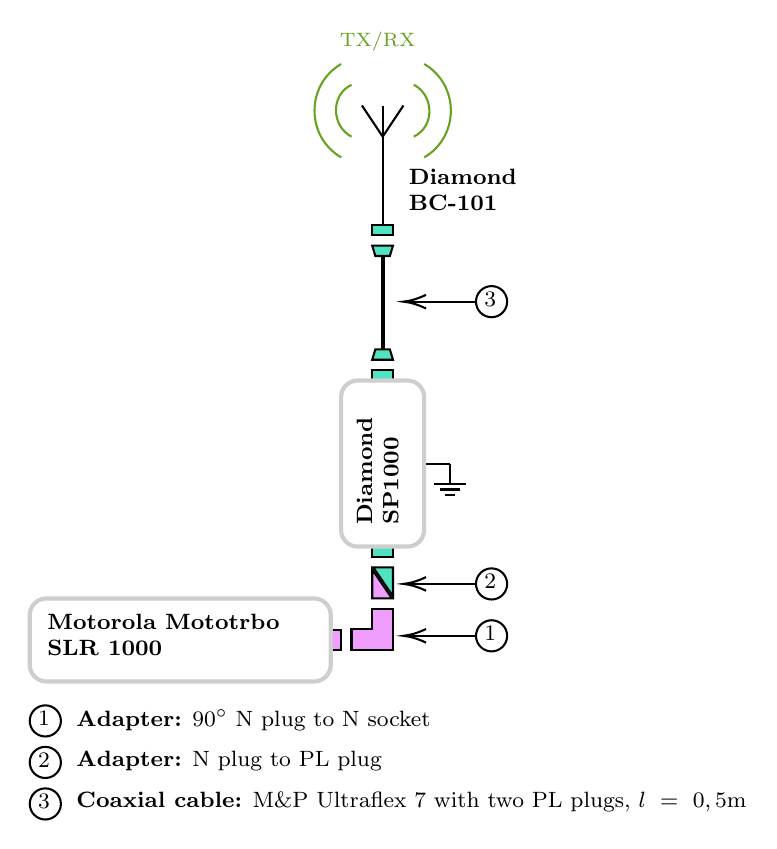
\begin{tikzpicture}[x=0.75pt,y=0.75pt,yscale=-1,xscale=1]
%uncomment if require: \path (0,463); %set diagram left start at 0, and has height of 463

%Straight Lines [id:da2117409366899652] 
\draw    (345,270) -- (357.5,270) ;
%Straight Lines [id:da19758281728068594] 
\draw    (357.5,270) -- (357.5,280) ;
%Straight Lines [id:da9706348152903634] 
\draw    (350,280) -- (365,280) ;
%Straight Lines [id:da9955066685628202] 
\draw    (352.5,282.5) -- (362.5,282.5) ;
%Straight Lines [id:da3542838525324348] 
\draw    (355,285) -- (360,285) ;

%Shape: Rectangle [id:dp5195215226134675] 
\draw  [fill={rgb, 255:red, 80; green, 227; blue, 194 }  ,fill opacity=1 ] (320,230) -- (320,225) -- (330,225) -- (330,230) -- cycle ;
%Shape: Rectangle [id:dp04379129192102571] 
\draw  [fill={rgb, 255:red, 80; green, 227; blue, 194 }  ,fill opacity=1 ] (320,315) -- (320,310) -- (330,310) -- (330,315) -- cycle ;
%Rounded Rect [id:dp609897861214854] 
\draw  [color={rgb, 255:red, 206; green, 206; blue, 206 }  ,draw opacity=1 ][line width=1.5]  (313,310) .. controls (308.58,310) and (305,306.42) .. (305,302) -- (305,238) .. controls (305,233.58) and (308.58,230) .. (313,230) -- (337,230) .. controls (341.42,230) and (345,233.58) .. (345,238) -- (345,302) .. controls (345,306.42) and (341.42,310) .. (337,310) -- cycle ;


%Straight Lines [id:da8216628264555428] 
\draw    (325.04,97.5) -- (325.04,157.5) ;
%Straight Lines [id:da11975977315738118] 
\draw    (315.04,97.5) -- (325.04,112.5) ;
%Straight Lines [id:da2623857929633875] 
\draw    (325.04,112.5) -- (335.04,97.5) ;
%Curve Lines [id:da9838947299311864] 
\draw [color={rgb, 255:red, 101; green, 162; blue, 30 }  ,draw opacity=1 ]   (340.04,87.5) .. controls (349.76,92.5) and (350.33,107.64) .. (340.04,112.5) ;
%Curve Lines [id:da48333252009100747] 
\draw [color={rgb, 255:red, 101; green, 162; blue, 30 }  ,draw opacity=1 ]   (345.04,77.5) .. controls (362.29,87.63) and (362.04,112.63) .. (345.04,122.5) ;

%Curve Lines [id:da06276736990916465] 
\draw [color={rgb, 255:red, 101; green, 162; blue, 30 }  ,draw opacity=1 ]   (310.04,112.5) .. controls (300.33,107.5) and (299.76,92.36) .. (310.04,87.5) ;
%Curve Lines [id:da8544747440552438] 
\draw [color={rgb, 255:red, 101; green, 162; blue, 30 }  ,draw opacity=1 ]   (305.04,122.5) .. controls (287.79,112.38) and (288.04,87.37) .. (305.04,77.5) ;

%Shape: Rectangle [id:dp5540086456806208] 
\draw  [fill={rgb, 255:red, 80; green, 227; blue, 194 }  ,fill opacity=1 ] (320.04,155) -- (330.04,155) -- (330.04,160) -- (320.04,160) -- cycle ;
%Shape: Rectangle [id:dp17515633991893775] 
\draw  [fill={rgb, 255:red, 239; green, 158; blue, 255 }  ,fill opacity=1 ] (300,350) -- (305,350) -- (305,360) -- (300,360) -- cycle ;
%Rounded Rect [id:dp7223835974557309] 
\draw  [color={rgb, 255:red, 206; green, 206; blue, 206 }  ,draw opacity=1 ][line width=1.5]  (155,343) .. controls (155,338.58) and (158.58,335) .. (163,335) -- (292,335) .. controls (296.42,335) and (300,338.58) .. (300,343) -- (300,367) .. controls (300,371.42) and (296.42,375) .. (292,375) -- (163,375) .. controls (158.58,375) and (155,371.42) .. (155,367) -- cycle ;


%Shape: Path Data [id:dp2172730430252452] 
\draw  [fill={rgb, 255:red, 239; green, 158; blue, 255 }  ,fill opacity=1 ] (310,360) -- (310,349.67) -- (320,349.67) -- (320,340) -- (330,340) -- (330,360) -- (310,360) -- cycle ;
%Shape: Right Triangle [id:dp30746565461403486] 
\draw  [fill={rgb, 255:red, 80; green, 227; blue, 194 }  ,fill opacity=1 ] (320.48,320) -- (330,333.98) -- (330,320) -- cycle ;
%Shape: Right Triangle [id:dp7515173690048442] 
\draw  [fill={rgb, 255:red, 239; green, 158; blue, 255 }  ,fill opacity=1 ] (329.52,335) -- (320,321.02) -- (320,335) -- cycle ;

%Straight Lines [id:da9120395561613033] 
\draw [line width=1.5]    (325,170) -- (325,215) ;
%Shape: Trapezoid [id:dp9006012786033941] 
\draw  [fill={rgb, 255:red, 80; green, 227; blue, 194 }  ,fill opacity=1 ][line width=0.75]  (330,165) -- (328.5,170) -- (321.5,170) -- (320,165) -- cycle ;
%Shape: Trapezoid [id:dp20960810518276118] 
\draw  [fill={rgb, 255:red, 80; green, 227; blue, 194 }  ,fill opacity=1 ][line width=0.75]  (320,220) -- (321.5,215) -- (328.5,215) -- (330,220) -- cycle ;

%Straight Lines [id:da35692414312633214] 
\draw    (370,353) -- (337,353) ;
\draw [shift={(335,353)}, rotate = 360] [color={rgb, 255:red, 0; green, 0; blue, 0 }  ][line width=0.75]    (10.93,-3.29) .. controls (6.95,-1.4) and (3.31,-0.3) .. (0,0) .. controls (3.31,0.3) and (6.95,1.4) .. (10.93,3.29)   ;
%Shape: Circle [id:dp44275798239943964] 
\draw   (370,353) .. controls (370,348.86) and (373.36,345.5) .. (377.5,345.5) .. controls (381.64,345.5) and (385,348.86) .. (385,353) .. controls (385,357.14) and (381.64,360.5) .. (377.5,360.5) .. controls (373.36,360.5) and (370,357.14) .. (370,353) -- cycle ;


%Shape: Circle [id:dp08416294362563437] 
\draw   (370,328) .. controls (370,323.86) and (373.36,320.5) .. (377.5,320.5) .. controls (381.64,320.5) and (385,323.86) .. (385,328) .. controls (385,332.14) and (381.64,335.5) .. (377.5,335.5) .. controls (373.36,335.5) and (370,332.14) .. (370,328) -- cycle ;

%Straight Lines [id:da011949664490807699] 
\draw    (370,328) -- (337,328) ;
\draw [shift={(335,328)}, rotate = 360] [color={rgb, 255:red, 0; green, 0; blue, 0 }  ][line width=0.75]    (10.93,-3.29) .. controls (6.95,-1.4) and (3.31,-0.3) .. (0,0) .. controls (3.31,0.3) and (6.95,1.4) .. (10.93,3.29)   ;

%Shape: Circle [id:dp29561759695484313] 
\draw   (370,192) .. controls (370,187.86) and (373.36,184.5) .. (377.5,184.5) .. controls (381.64,184.5) and (385,187.86) .. (385,192) .. controls (385,196.14) and (381.64,199.5) .. (377.5,199.5) .. controls (373.36,199.5) and (370,196.14) .. (370,192) -- cycle ;

%Straight Lines [id:da6708191132816714] 
\draw    (370,192) -- (337,192) ;
\draw [shift={(335,192)}, rotate = 360] [color={rgb, 255:red, 0; green, 0; blue, 0 }  ][line width=0.75]    (10.93,-3.29) .. controls (6.95,-1.4) and (3.31,-0.3) .. (0,0) .. controls (3.31,0.3) and (6.95,1.4) .. (10.93,3.29)   ;

%Shape: Circle [id:dp6925244802161248] 
\draw   (155,394) .. controls (155,389.86) and (158.36,386.5) .. (162.5,386.5) .. controls (166.64,386.5) and (170,389.86) .. (170,394) .. controls (170,398.14) and (166.64,401.5) .. (162.5,401.5) .. controls (158.36,401.5) and (155,398.14) .. (155,394) -- cycle ;

%Shape: Circle [id:dp5144865887931986] 
\draw   (155,414) .. controls (155,409.86) and (158.36,406.5) .. (162.5,406.5) .. controls (166.64,406.5) and (170,409.86) .. (170,414) .. controls (170,418.14) and (166.64,421.5) .. (162.5,421.5) .. controls (158.36,421.5) and (155,418.14) .. (155,414) -- cycle ;

%Shape: Circle [id:dp2881120818061964] 
\draw   (155,434) .. controls (155,429.86) and (158.36,426.5) .. (162.5,426.5) .. controls (166.64,426.5) and (170,429.86) .. (170,434) .. controls (170,438.14) and (166.64,441.5) .. (162.5,441.5) .. controls (158.36,441.5) and (155,438.14) .. (155,434) -- cycle ;



% Text Node
\draw (157.5,428) node [anchor=north west][inner sep=0.75pt]  [font=\footnotesize] [align=left] {3};
% Text Node
\draw (157.5,408) node [anchor=north west][inner sep=0.75pt]  [font=\footnotesize] [align=left] {2};
% Text Node
\draw (157.5,388) node [anchor=north west][inner sep=0.75pt]  [font=\footnotesize] [align=left] {1};
% Text Node
\draw (372.5,186) node [anchor=north west][inner sep=0.75pt]  [font=\footnotesize] [align=left] {3};
% Text Node
\draw (372.5,322) node [anchor=north west][inner sep=0.75pt]  [font=\footnotesize] [align=left] {2};
% Text Node
\draw (372.5,347) node [anchor=north west][inner sep=0.75pt]  [font=\footnotesize] [align=left] {1};
% Text Node
\draw (302.89,60.5) node [anchor=north west][inner sep=0.75pt]  [font=\scriptsize,color={rgb, 255:red, 101; green, 162; blue, 30 }  ,opacity=1 ] [align=left] {TX/RX};
% Text Node
\draw (311,301) node [anchor=north west][inner sep=0.75pt]  [font=\footnotesize,rotate=-270] [align=left] {\textbf{Diamond}\\\textbf{SP1000}};
% Text Node
\draw (162,341) node [anchor=north west][inner sep=0.75pt]  [font=\footnotesize] [align=left] {\textbf{Motorola Mototrbo}\\\textbf{SLR 1000}};
% Text Node
\draw (336.2,126.5) node [anchor=north west][inner sep=0.75pt]  [font=\footnotesize] [align=left] {\textbf{Diamond }\\\textbf{BC-101}};
% Text Node
\draw (176,427) node [anchor=north west][inner sep=0.75pt]  [font=\footnotesize] [align=left] {\textbf{Coaxial cable:} M\&P Ultraflex 7 with two PL plugs, $\displaystyle l\ =\ 0,5\mathrm{m}$};
% Text Node
\draw (176,407) node [anchor=north west][inner sep=0.75pt]  [font=\footnotesize] [align=left] {\textbf{Adapter:} N plug to PL plug};
% Text Node
\draw (176,387) node [anchor=north west][inner sep=0.75pt]  [font=\footnotesize] [align=left] {\textbf{Adapter:} $\displaystyle 90^{\circ }$ N plug to N socket};


\end{tikzpicture}

	\caption{Schematic structure of repeater radio infrastructure.}
	\label{fig:tikz_repeater}
\end{figure}

Using the specifications of the SLR 1000 listed in the table \ref{tab:table_slr1000_specs}, the maximum transmission power is calculated in the equation (\ref{eq:power_rep_tx}). The minimum required reception power for the worst case can be taken from the equation (\ref{eq:power_BSt_min}).
\begin{table}[h!] % SLR1000
	\centering
	\footnotesize
\begin{tabular}{|l|c|}
	\hline
	\multicolumn{2}{|c|}{\textbf{Motorola Mototrbo SLR 1000 (VHF digital) specifications}} \\
	\hline
 	Frequency & $136\mathrm{MHz}$ to $174\mathrm{MHz}$ \\
	System impedance & $50\Omega$\\
 	Dimensions $\mathrm{(H \times W \times D)}$ & $279 \times 229 \times 102 \mathrm{mm}$ \\%
 	Mass & $4,54\mathrm{kg}$ \\%
	Power supply & $12\mathrm{VDC}$ ($11,0$ to $15,5\mathrm{VDC}$) \\
	Current RX and standby & $0,7\mathrm{A}$ ($0,63\mathrm{A}$ typical) \\
	Current TX & $3\mathrm{A}$ (max.) \\
	Operating temperature & $-30^\circ \mathrm{C}$ to $60^\circ \mathrm{C}$ \\
	RX sensitivity 5\% BER: & $0,25\mathrm{\mu V}$ ($0,18\mathrm{\mu V}$ typical) \\
	TX power output & $1\mathrm{W}$ to $10\mathrm{W}$ \\
	Connector & N socket\\
	IP rating & $65$\\
	\hline
\end{tabular}
	\caption{Excerpt from the data sheet of the Motorola Mototrbo SLR 1000 repeater. \cite{SLR1000:2019}}
	\label{tab:table_slr1000_specs}
\end{table}
\begin{equation} \label{eq:power_rep_tx}
	\centering
	P_\mathrm{T,dBW} =  10\mathrm{dBW} \cdot \log_{10} \left( \dfrac{10\mathrm{W}}{1\mathrm{W}} \right) = 10\mathrm{dBW}\text{,}
\end{equation}

Since the repeater uses the same lightning arrester and the same antenna as the base station, the resulting losses can be taken directly from the equations (\ref{eq:losses_BSt_arr}) and (\ref{eq:losses_BSt_ant}). The antenna of the repeater is always mounted at a height of $h_\mathrm{REP} = 8\mathrm{m}$ above the ground, as a mast is included in the system design. 

As can be seen in the figure \ref{fig:tikz_repeater}, the length of the coaxial cable is $0,5\mathrm{m}$, resulting in an insertion loss of:   
\begin{equation} \label{eq:losses_BSt_coax}
	\centering
	L_\mathrm{coax,dB} = \dfrac{7,2471 \cdot 0,5}{100}\mathrm{dB} = 0,036\mathrm{dB}\text{.}
\end{equation}

With the number of adapters and connectors $N_\mathrm{I} = 4$, their insertion loss follows to:
\begin{equation} \label{eq:losses_rep_conn}
	\centering
	L_\mathrm{conn/adapt,dB} = 0,4\mathrm{dB}\text{.}
\end{equation}

Finally, the total loss of the antenna feed line can be calculated with:
\begin{equation} \label{eq:losses_rep}
	\centering
	L_\mathrm{REP,dB} = L_\mathrm{arr,dB} + L_\mathrm{ant,dB} + L_\mathrm{coax,dB} + L_\mathrm{conn/adapt,dB} = 0,849\mathrm{dB}\text{.}
\end{equation}
